%!TEX root=paper.tex

% \newpage
\section{What is the Perception of the Learners?}
\label{sec:perception}

\subsection{Post-Usage Survey}

After the semester was over, we sent an email to the students, asking them to answer several questions about their experience. Our survey was answered by \surveyrespondents students in total. Figure \ref{fig:reader_use} shows that most of the respondents found the system easy to use and useful. 

 \begin{figure}[h!]
    \centering
      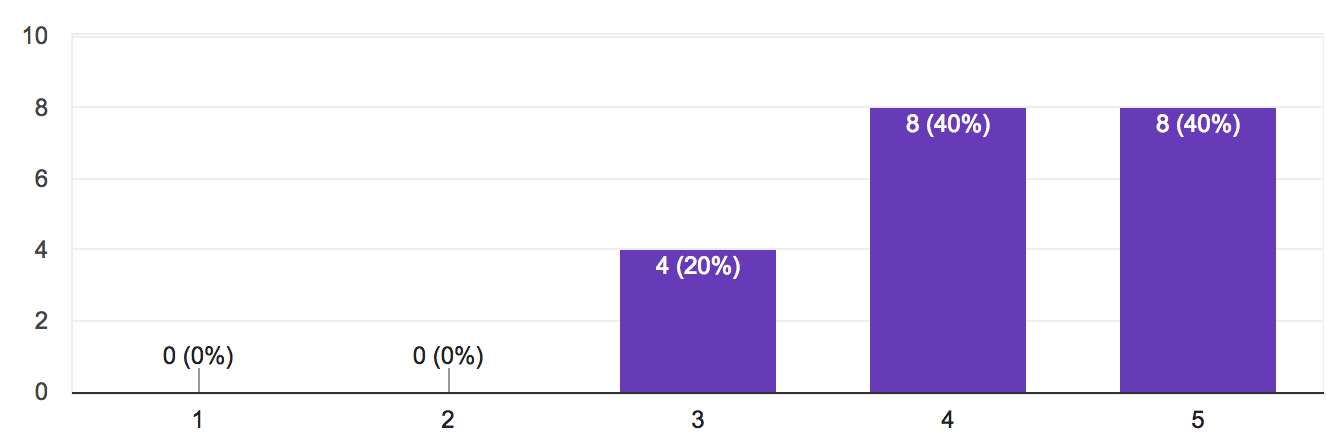
\includegraphics[width=0.8\columnwidth]{figures/opinions/reader_ease_of_use}
      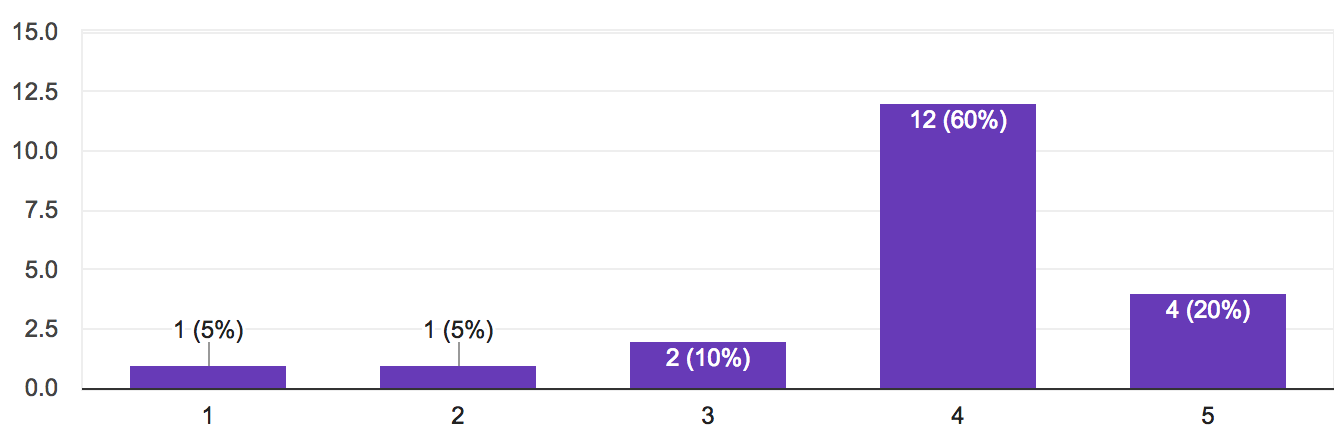
\includegraphics[width=0.8\columnwidth]{figures/opinions/reader_usefulness}
      \caption{Student assessment of ease of use (top) and usefulness (bottom) of the reader}
      \label{fig:reader_use}
    \end{figure}

We asked the participants what would make their experience better. Many thought that the system was good the way it was, and a few others had some more specific answers (e.g. night reading mode, etc.). \footnote{The complete feedback is available in the GitHub repository of the paper.}. The most requiring requests were: 

\begin{itemize}
	\item Choice of Topics: 
		\squote{Order in different subjects like animals, politics, fashion...}, 
		\squote{Add a choice for different topics not only for the sources}, 
		\squote{Better display of the articles and tags such as 'gaming' or 'news'}, etc.
	\item More freedom for chosing materials: 
		\squote{Would be nice to be able to add website to the list} and 
		\squote{A search engine}. 
\end{itemize}

When asked about what they dislike about the Reader, the majority of feedback was related to translations: two people complained about them being in English (\squote{The translations are always in English}), five people complained about the translation quality (e.g. \squote{Some weak translations}). The English translations are the reason for which one learner reported that they prefer the textbook: \squote{The translations are always in English. This is why I would grab a textbook first. I don't want to look up the (English to) Dutch translation.}

Figure \ref{fig:ex_rating} shows that when asked to provide their personal rating of the the quality of the exercises, the majority of the respondents expresses their appreciation. 

 \begin{figure}[h!]
    \centering
      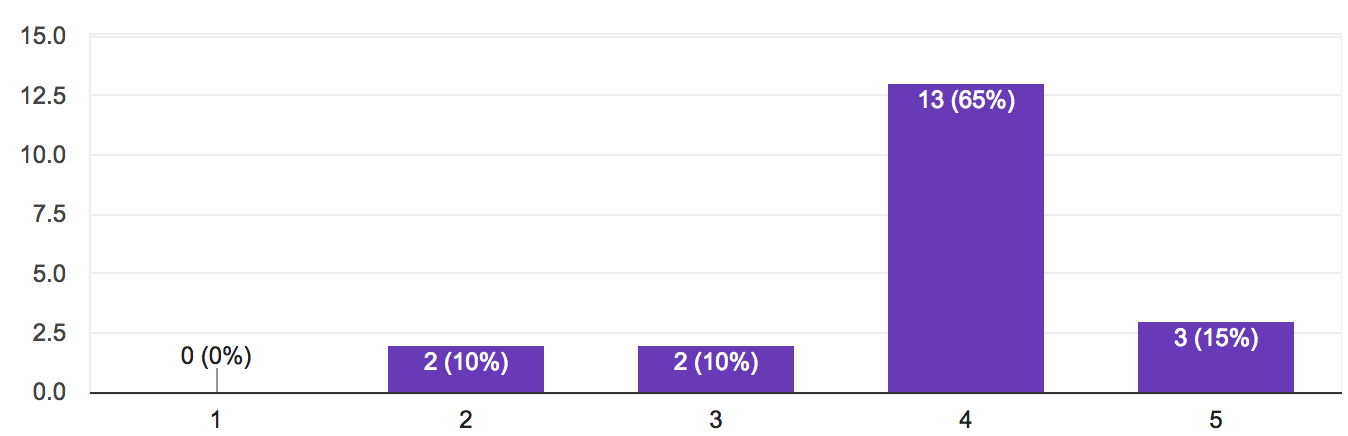
\includegraphics[width=0.8\columnwidth]{figures/opinions/exercises_rating}
      \caption{Students assessment  of the generated exercises}
      \label{fig:ex_rating}
    \end{figure}

When asked about what they dislike about exercises, many said literally ``nothing''. However, several also had concrete feedback: 
\begin{itemize}
	\item During exercises, translations are disabled, so if one does not understand a word from the context, they will have a difficulty.
		\squote{There aren't translations},
		\squote{Doesn't give the translations}
	\item Difficulty is not always appropriate: \squote{Some exercises are too easy}
	\item Contexts are always the same: \squote{I would like to see the words I practice in a different context}
\end{itemize}

Finally, we asked whether our learners would prefer our system to a textbook if offered the choice. We thus asked them what would they choose between the our system (Zeeguu Reader in the figure) and a textbook. We also gave them the possibility to answer something else with a free-form text field. Figure \ref{fig:preferred_reader} shows that the majority of the learners who answered our post-usage survey would prefer our system. However, some still prefer a textbook. 

 \begin{figure}[h!]
    \centering
      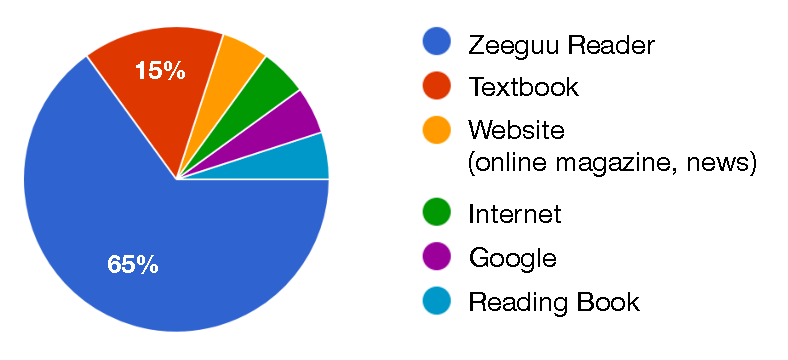
\includegraphics[width=0.8\columnwidth]{figures/opinions/reader_vs_textbook}
      \caption{Answers to the question: {\em ``If you wanted to read something in the language you study, what would you reach out for first?''}}
      \label{fig:preferred_reader}
    \end{figure}



\subsection{In-App Feedback}
Besides the analysis  based on the observed telemetry data, we also asked the students a series of questions by popping up questions while they were using the system. To do this, we used an online tool called HotJar. Among the questions was whether they preferred the reading platform and why. Some of the answers can be seen in the screenshot below. It becomes clear that the students appreciate the possibility of reading what is interesting for them.

    \begin{figure}[h!]
    \centering
      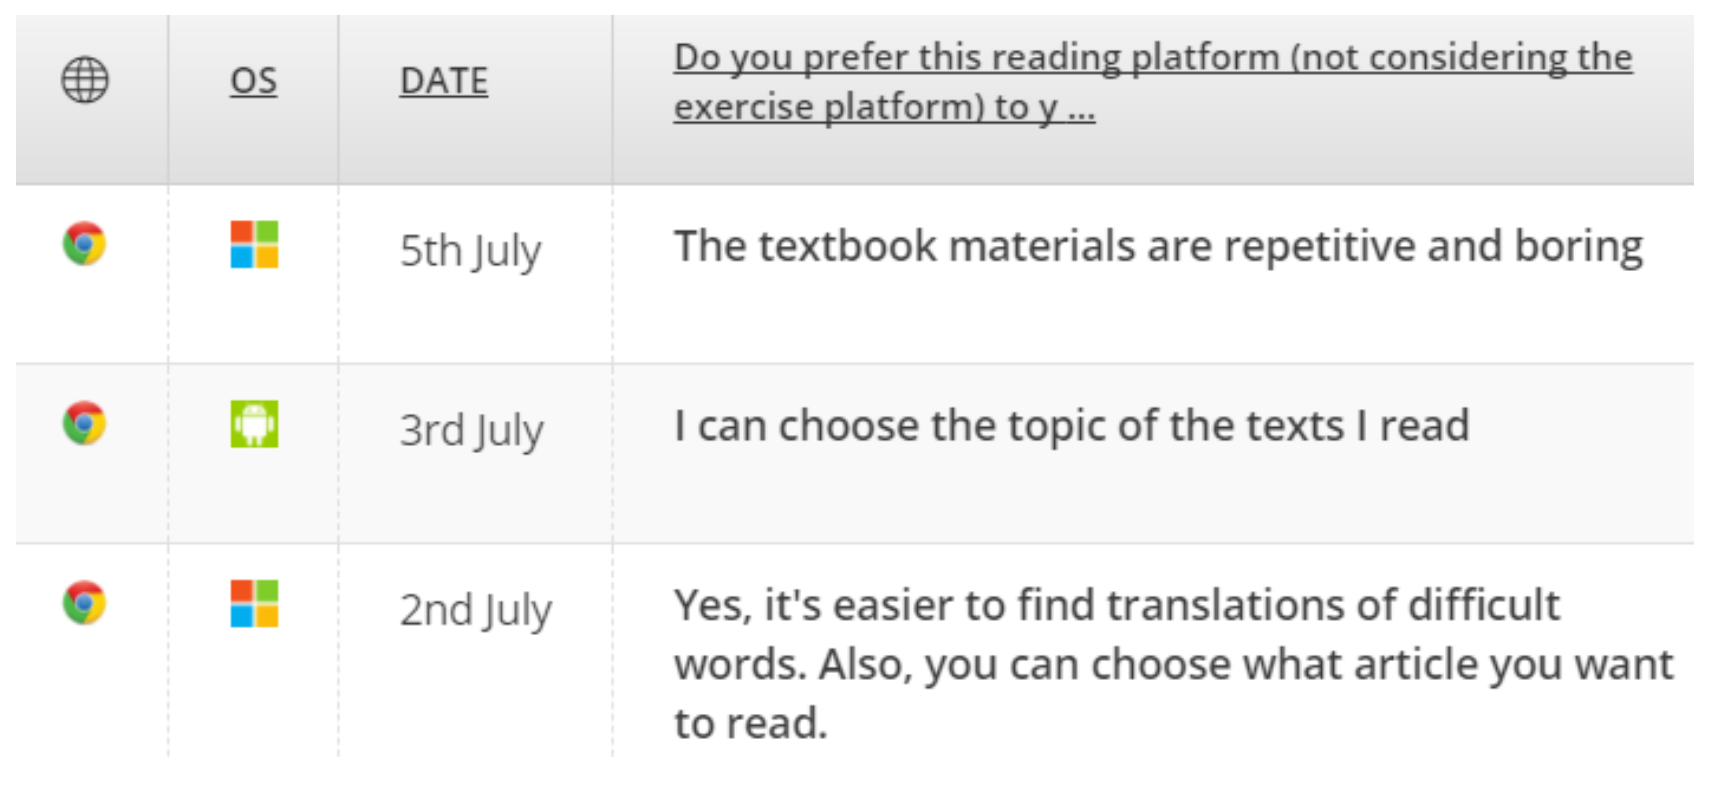
\includegraphics[width=0.9\columnwidth]{figures/opinion_on_reading_platform}
      \caption{The students appreciate the freedom of choosing what to read}
    \end{figure}


% \newpage
\subsection{Reports to the Teacher}
To triangulate the answers that they provided to us, we report here also what the students wrote in a separate evaluation of the tools they use in the class, which the teacher runs always at the end of the school year. Several of the answers are: 

\begin{description}
  \item {\em ``It works well but it were better if the translation would have been in Dutch. It is good that you can choose what to read.''}
  \item {\em ``Good for reading skills. Would have been best if it were in Dutch.''}
  \item {\em ``Your vocabulary is really moving forward, but then you have to do it more often than a few times. Overall a nice website, easy and fun subjects''}
\end{description}

The main message in the feedback is that learners appreciate the freedom of choosing materials to read that are personally interesting for them. The second implied observation is that they appreciate the translations, but they would want to have them in their native language. 


% The way forward is then, by providing better recommendations if possible, and by providing translations in their native languages.

% In the future we plan to investigate whether the system works well enough with Dutch.
